% Technische Universität Dresden
% Fakultät Informatik
% Institut für Software- und Multimediatechnik
% Seniorprofessur für Multimediatechnik
%
% Example document demonstrating the usage of mmthesis.sty
% 2012-10-26 Andreas Rümpel
% 
% ### build hints (% = filename of tex file) ###
% pdflatex: pdflatex %.tex
% biber: biber % (biber is a modern backend for bibtex, http://biblatex-biber.sourceforge.net)
% glossaries and acronyms: makeglossaries %
%
% Das LATEX2e-Sündenregister: ftp://ftp.dante.de/tex-archive/info/l2tabu/german/l2tabu.pdf
% KOMAScript-Guide: ftp://ftp.dante.de/tex-archive/macros/latex/contrib/koma-script/scrguide.pdf
% Einige typographische Grundregeln und ihre Umsetzung in LaTeX: http://www2.informatik.hu-berlin.de/sv/lehre/typographie.pdf

\documentclass[
	headsepline,
	footsepline,
	fontsize=12pt,
	%draft, % use this for finding overfull boxes
	%parskip, % use this for alternative paragraph formatting
	bibliography=totoc
]{scrbook}


\usepackage[utf8]{inputenc}
\usepackage{mmthesis}
\addbibresource{library.bib} % put name of bib file here with extension

%### switches
%\printoutput % make link colors black, leave deactivated for screen output

%### define metadata
\mmtype{Diplomarbeit} %Diplomarbeit|Großer Beleg|Bachelorarbeit|Masterarbeit|Seminararbeit
\mmtitle{Semantik-gestütztes Hilfesystem für ein komposites Informationsvisualisierungssystem}
\mmtshorttitle{Hilfesystem für komposite InfoVis}
\mmtauthor{Nikolaus Piccolotto}
\mmtsubmissionmonth{November 2013}
\mmtsubmissiondate{30. November 2013}
\mmtsupervisor{Dipl.-Medieninf. Martin Voigt}
%\mmtsupervisorii{Dipl.-Medieninf. Foo Bar} % Co-supervisor, optional

\mmthypersetup % has to be called after setting metadata

%### acronyms
\newacronym{PDF}{PDF}{Portable Document Format}
\newacronym{RCP}{RCP}{Rich Client Platform}
\newacronym{RIA}{RIA}{Rich Internet Application}
\newacronym{RELAXNG}{RELAX NG}{Regular Language Description for XML New Generation}
\newacronym{SGML}{SGML}{Standard Generalized Markup Language}
\newacronym{SWT}{SWT}{Standard Widget Toolkit}
\newacronym{WDC}{W3C}{World Wide Web Consortium}
\newacronym{WPF}{WPF}{Windows Presentation Foundation}
\newacronym{XPath}{XPath}{XML Path Language}
\newacronym{XHTML}{XHTML}{Extensible Hypertext Markup Language}
\newacronym{XML}{XML}{Extensible Markup Language}
% my acronyms
\newacronym{InfoVis}{InfoVis}{Informationsvisualisierung}

\begin{document}
\frontmatter
\pagenumbering{Roman}
\mmtfrontmatter

\listoffigures
\listoftables
\printglossary[type=\acronymtype,style=long,title=Abkürzungsverzeichnis,toctitle=Abkürzungsverzeichnis]
%\printglossary %Glossar

\mainmatter

\chapter{Einleitung}
\label{chapter:einleitung}

% Hier kommt eine kurze Einführung von semantischen Daten, nehme ich an

\section{Motivation}
\label{section:motivation}

% Hier wird generell eingeleitet, also vermutlich die Problematik zwischen semantischen Datensätzen und Endusern

\section{Problemstellung und Zielsetzung}
\label{section:problemstellung}

% Hier wird quasi der Vizboard Workflow umrissen
% und erklärt, wo das eigentliche Problem liegt, nämlich im Information Overload beim letzten Schritt

\begin{figure}[htbp]
	\centering
	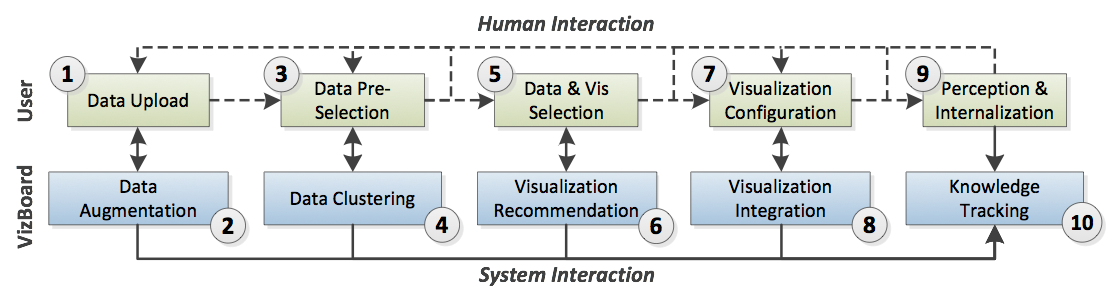
\includegraphics[width=0.75\textwidth]{images/vizboard_workflow.png}
	\caption{VizBoard Workflow}
	\label{figure:vizboard_workflow}
\end{figure}

\section{Aufbau der Arbeit}
\label{section:aufbau}

% Aufbau der Arbeit erklären, kommt zum Schluss

\chapter{Stand der Forschung und Technik}
\label{chapter:standderforschung}

\section{Grundlagen}
\label{section:grundlagen}

\section{Szenario}
\label{section:szenario}

% kurze einleitung noch mal

Wie in Kapitel~\ref{chapter:einleitung} erläutert, ist das komposite InfoVis-System Teil der Anwendung VizBoard. Sie leitet den Benutzer in mehreren Schritten von der Auswahl eines Datensatzes zur finalen, kompositen Informationsvisualisierung. Im vorletzten Schritt wählt dieser mit Hilfe eines Facettenbrowsers geeignete Visualisierungskomponenten aus, welche danach angezeigt werden. Um die Problemstellung noch einmal zu verdeutlichen, wird im folgenden ein mögliches Szenario beschrieben.

% einführung der problemstellung
Alice möchte für ihr Biologiestudium mehr über die geografische Verteilung verschiedener Genvarationen herausfinden. Dazu sucht sie im Internet nach einem Datensatz, welchen sie auch findet. Leider ist er in einem für Alice unbekannten Format abgespeichert, nämlich OWL. Außerdem ist er ca. 30\,MB groß, das ist zu viel um es manuell zu verarbeiten. Davon abgesehen sind geografische Breite und Länge als Zahlenkombination keine anschauliche Repräsentation von Orten. Alice hört von einem Freund, dass VizBoard gut geeignet ist um semantische Datensätze anzusehen und probiert es aus.

% Der Benutzer ist laut unserem Rollenmodell weder Developer noch Visualisierungsexperte, d.h. er hat erstmal Schwierigkeiten zu erfassen, was hier überhaupt abgeht

Nachdem Alice ihren Datensatz auch bei VizBoard gefunden und die gewünschten Visualisierungskomponenten (eine Karte, ein Balkendiagramm, eine Tabelle und eine Treemap) ausgewählt hat, werden diese ihr angezeigt. Alice benutzt VizBoard zum ersten Mal und macht außer Facebook und YouTube auch sonst nicht viel im Internet, das heißt sie ist zunächst von den vier unterschiedlichen Fenstern etwas überfordert.

VizBoard bietet Alice aber sofort eine einführende Übersicht und erklärt kurz die Darstellungsform und den Inhalt jeder Komponente. Eine denkbare Erklärung der Treemap wäre zum Beispiel:

\begin{quote}
Eine Treemap ist eine hierarchische Visualisierung um Größenverhältnisse anschaulich zu machen. In dieser werden die Anzahl von Genvariationen pro geografischer Region dargestellt.
\end{quote}

% Was sind das für Fenster? Welche Komponente ist welche? Welche macht was? Wie kann ich sie bedienen? HUUUPS da ändert sich ja was obwohl ich dort nix gemacht hab! Wie hängen die zusammen? Was sind das für Daten, die dargestellt werden? 

Damit bekommt Alice einen Überblick über die verfügbaren Visualisierungen und weiß, welches Fenster welche Visualisierung enthält und für was diese gut sind. Nun möchte sie die Tabelle, in der die durch die Treemap visualisierten Daten stehen, nach der Spalte \enquote{Anzahl} sortieren. Alice sieht aber nicht, wie sie das machen soll, da in der Tabelle kein offensichtliches Kontrollelement wie z.\,B. ein Button vorhanden ist. Sie bemerkt ein Fragezeichen in der Titelleiste des Fensters und klickt darauf. Der verfügbare Viewport wird abgedunkelt und es erscheint ein neues Fenster, welches die verfügbaren Aktionen mit Hilfe von Text, Bildern und Animationen erklärt. Alice lernt, dass sie mit einem einfachen Linksklick auf den jeweiligen Kopf einer Tabellenspalte nach dieser sortieren kann und außerdem eine oder mehrere Zeilen auswählen kann. Sie sortiert die Tabelle wie gewollt und wählt die ersten drei Zeilen aus. Plötzlich verkleinert die Karte ihr Zoomlevel und Alice ist verwirrt: Sie hat nur mit der Tabelle interagiert und es bestand keine sichtbare Verbindung zwischen den beiden Fenstern. Allerdings wurde nach der Zeilenauswahl ein Pfeil von der Tabelle zur Karte gezeichnet, welcher mit einem Icon in Form eines Briefes versehen ist. Alice vermutet, dass doch irgendeine Verbindung zwischen den beiden Visualisierungen besteht und klickt auf den Brief. Ähnlich wie vorhin bei der Hilfe zur Tabelle wird der Viewport abgedunkelt und ein neues Fenster wird eingeblendet. Es erklärt die Kommunikation zwischen den Visualisierungen mit Hilfe von Animationen, Text und Bildern. Nun weiß Alice auch, wie die verschiedenen Fenster zusammenhängen und kann sich ihrer eigentlichen Aufgabe widmen.

% Was heißt GDP? Wie wird das berechnet? Was soll die Spitze bei 1990? Woher kommt die? Diese eine Komponente scheint kaputt zu sein, wo kann ich mich beschweren?

In der Tabelle findet sie auch eine Spalte \enquote{SNP}. Alice weiß zwar, dass sie die Abkürzung schon einmal gesehen hat, kennt aber im Moment ihre Bedeutung nicht. Praktischerweise ist der Spaltenkopf mit der Wikipedia verlinkt und sie wird sofort auf die entsprechende Seite weitergeleitet. Alice erinnert sich, dass \enquote{SNP} \enquote{Single-nucleotide polymorphism} bedeutet und sie bekommt auch gleich zusätzliche Informationen zu diesem Thema. Sie widmet sich weiter der Tabelle und stellt fest, dass die Ortsbezeichnung \enquote{Kopenhagen} nicht mit der Markierung in der Karte übereinstimmt. Außerdem ist sie erstaunt, wie hoch die Verbreitung eines bestimmten SNPs dort ist und würde gerne die Ursache dafür wissen. In der Hilfe zur Tabelle wurde sie auch über die Möglichkeit, Kommentare an den Daten vorzunehmen, aufgeklärt. Alice kommentiert sowohl die falschen Geokoordinaten als auch ihre Frage über die Verbreitung des SNPs, sodass sie später per Email über Antworten informiert wird. Nun kann Alice sich mit der vierten Visualisierung, dem Balkendiagramm, beschäftigen. Allerdings reagiert es auf keine Mausklicks und macht auch sonst nicht den Eindruck, die Daten akkurat darzustellen. Alice meldet die kaputte Visualisierung über die eingebaute Reporting-Funktion und schließt das Fenster, um sich den anderen drei Visualisierungskomponenten zuzuwenden.

\chapter{Konzept}

\section{Anforderungsanalyse}
\label{section:anforderungsanalyse}

Aus dem Szenario (Kapitel~\ref{section:szenario}) lassen sich nun verschiedene Anforderungen an ein Hilfesystem für komposite Informationsvisualisierungssysteme ableiten.

\subsection{Funktionale Anforderungen}
\label{section:funktionale_anforderungen}

Blabla

\begin{itemize}
	\item\textbf{Überblick}: Das Hilfesystem soll einen kurzen Überblick über das InfoVis-System geben und Darstellungsform sowie Inhalt jeder Komponente kurz erläutern.
	\item\textbf{Bedienung}: Das Hilfesystem soll erklären können, wie eine Komponente bedient wird. Diese Informationen umfassen beispielsweise welche Operationen welche Aktionen (eventuell auf welchen Daten) ausführen.
	\item\textbf{Reporting}: Fehler in Komponenten sollen über ein Reporting-System gemeldet werden können.
	\item\textbf{Verlinkung}: Das Hilfesystem soll nicht-triviale Begriffe mit der Wikipedia verlinken, sodass nicht nur auf die Begriffsbedeutung hingewiesen werden, sondern dem Benutzer auch zusätzliche Informationen zur Verfügung gestellt werden können.
	\item\textbf{Kommunikation}: Das Hilfesystem soll erklären können, wie gegebene Komponenten miteinander kommunizieren.
	\item\textbf{Kommentare}: Der Benutzer soll die Möglichkeit haben Daten zu kommentieren und Bereiche der Visualisierung zu markieren und mit ebenfalls mit einem Kommentar zu versehen, sodass auch auf fehlende Daten hingewiesen werden kann.
\end{itemize}

\subsection{Nichtfunktionale Anforderungen}
\label{section:nichtfunktionale_anforderungen}

Bla bla

\begin{itemize}
	\item\textbf{Korrektheit}: Eine gegebene Hilfestellung darf keine Fehlinformationen enthalten, weil sie sonst mehr verwirrt als hilft.
	\item\textbf{Vollständigkeit}: Eine gegebene Hilfestellung muss alle Informationen enthalten, die der Nutzer benötigt um danach seine gewünschte Aufgabe ausführen zu können.
	\item\textbf{Verständlichkeit}: Hilfestellungen müssen in einer Form präsentiert werden, die der Benutzer schnell und mit geringem mentalen Aufwand verarbeiten kann.
	\item\textbf{Einheitlichkeit}: Das Look \& Feel von Teilen des Hilfesystems (z.B. Kommentare) muss komponentenübergreifend einheitlich sein, damit der Benutzer einmal gelerntes wiederverwenden kann.
	\item\textbf{Minimalität}: Der Komponentenentwickler soll seine Komponente mit möglichst wenig Aufwand zum Hilfesystem kompatibel machen können, ansonsten werden nur sehr wenige Komponenten -- und damit der Benutzer -- davon profitieren.
	\item\textbf{Universalität}: Das Hilfesystem soll für alle Komponenten und Visualisierungen in gleicher Qualität funktionieren.
	\item\textbf{Wiederverwendbarkeit}: Die Kommentare sollen möglichst in allen Visualisierungen wiederverwendet werden, damit viele Benutzer von den Erkenntnissen anderer profitieren können.
	\item\textbf{Unaufdringlichkeit}: Das Hilfesystem soll den Benutzer nicht von seinen Aufgaben ablenken und nur auf Anfrage zum Einsatz kommen oder es soll selbständig erkennen, wenn der Benutzer Hilfe benötigt.
\end{itemize}

%### end of appendix
%#####################################################
\printbibliography[title=Literaturverzeichnis]

%\printindex

\end{document}